\section{Experiments}
% We assess the effectiveness of our methods by exploring the following research questions:

% \textbf{RQ1.} Do the proposed methods offer any advantages over previous works?

% \textbf{RQ2.} How is the quality of auto-constructed Law-Graph?

% \textbf{RQ3.} Is the new design essential when we have Large Language Models? 

\subsection{Experimental Setup} \label{es}
\paragraph{Datasets.} The Chinese AI and Law Challenge 2018 (CAIL2018) is widely utilized in the Legal Judgment Prediction (LJP) task \cite{DBLP:journals/corr/abs-1807-02478}\footnote{All cases come from China Judgment Online. All personal information has already been hidden.}. In this paper, we specifically focus on four Crimes: \textit{fraud}, \textit{intentional injury}, and \textit{arson}. These four crimes are defined by Articles 193, 234, and 114 of the Criminal Acts of China, respectively. To evaluate the predictive capabilities of models across varying training case sizes, we randomly selected cases as the training sets, with sizes ranging from 10 to 1,000 cases. To reduce randomness, we performed five times of random selection. Table~\ref{tab:test} details the statistical outcomes for the test sets of these crimes.

\begin{table}
    \centering
    \scriptsize
    \caption{Statistical test cases for the Crime of fraud, intentional injury, and Arson. 
    %where '\#Cases' represents the number of cases. 
    According to these legal provisions, we divide these cases into three categories: 0 to 3 years, 3 to 10 years, and more than 10 years.}
    \begin{tabular}{ccccc}
    \toprule
      Crime & \#Cases & 0 to 3 & 3 to 10&More than 10\\
      \hline \vspace{-2mm} \\
    Fraud & 6004 & 3265 & 2186 & 553\\
    Intentional Injury & 8148 & 5110 & 2632 & 406\\
    % Robbery & 777 & 0 & 689 & 88\\
    Arson & 510 & 121 & 369 & 20\\
    \bottomrule
    \end{tabular}
    \label{tab:test}
\end{table}

\begin{figure*}
\vspace{-2em}

    \centering
% \vfill
\subfigure[Fraud: RMSE]{\label{fig:fraud-rmse}
\includegraphics[width=0.3\linewidth]{figs/fraud-rmse.png}}
\hspace{0.001\linewidth}
\subfigure[Fraud: Macro F1]{\label{fig:fraud-f1}
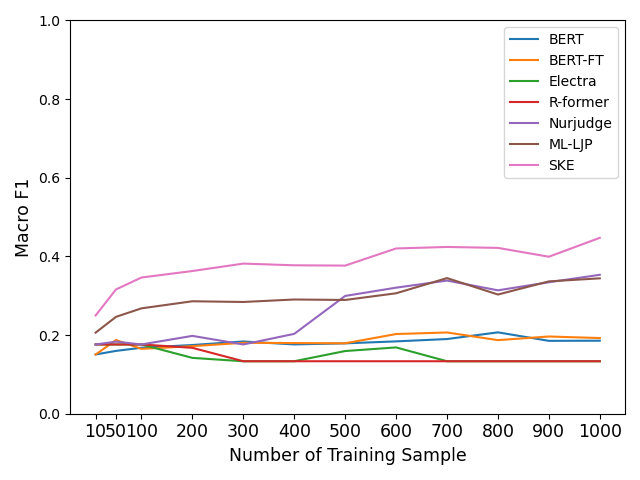
\includegraphics[width=0.3\linewidth]{figs/fraud-F1.png}}
\hspace{0.001\linewidth}
\subfigure[Fraud: Pearson]{\label{fig:fraud-p}
\includegraphics[width=0.3\linewidth]{figs/fraud-pearson.png}}
\vspace{-1em}

\vfill
\hspace{0.001\linewidth}
\subfigure[Intentional Injury: RMSE]{\label{fig:injure-rmse}
\includegraphics[width=0.3\linewidth]{figs/injure-rmse.png}}
\hspace{0.001\linewidth}
\subfigure[Intentional Injury: Macro F1]{\label{fig:injure-f1}
\includegraphics[width=0.3\linewidth]{figs/injure-F1.png}}
\hspace{0.001\linewidth}
\subfigure[Intentional Injury: Pearson]{\label{fig:injure-p}
\includegraphics[width=0.3\linewidth]{figs/injure-pearson.png}}
    \vspace{-1em}

% \vfill
% \hspace{0.001\linewidth}
% \subfigure[Robbery: RMSE]{\label{fig:robbery-rmse}
% \includegraphics[width=0.3\linewidth]{figs/robbery-rmse.png}}
% \hspace{0.001\linewidth}
% \subfigure[Robbery: Macro F1]{\label{fig:robbery-f1}
% \includegraphics[width=0.3\linewidth]{figs/robbery-F1.png}}
% \hspace{0.001\linewidth}
% \subfigure[Robbery: Pearson]{\label{fig:robbery-p}
% \includegraphics[width=0.3\linewidth]{figs/robbery-pearson.png}}
%         \vspace{-1em}

\vfill
\hspace{0.001\linewidth}
\subfigure[Arson: RMSE]{\label{fig:arson-rmse}
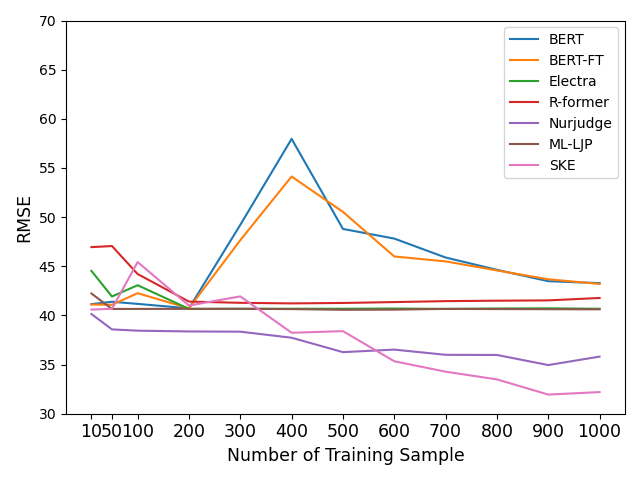
\includegraphics[width=0.3\linewidth]{figs/arson-rmse.png}}
\hspace{0.001\linewidth}
\subfigure[Arson: Macro F1]{\label{fig:arson-f1}
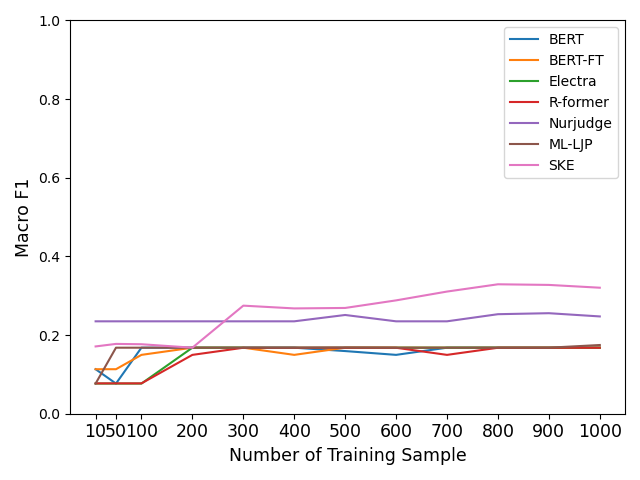
\includegraphics[width=0.3\linewidth]{figs/arson-F1.png}}
\hspace{0.001\linewidth}
\subfigure[Arson: Pearson]{\label{fig:arson-p}
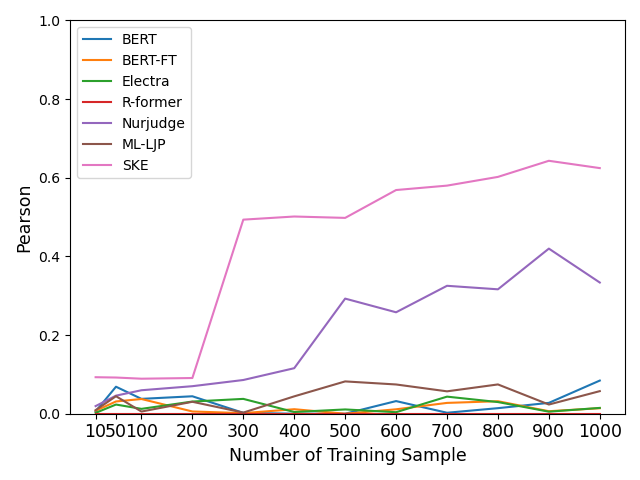
\includegraphics[width=0.3\linewidth]{figs/arson-pearson.png}}
    \vspace{-1em}

\caption{Results on Three Different Crimes.
% \Kaiqi{Perhaps report 3 datasets instead of 4. We shouldn't use one page for a figure.}
}
\label{fig:over}
\vspace{-0.5em}
\end{figure*}

\paragraph{Baselines.}
We compare with the following baseline models: (1) Language models: Both BERT~\cite{devlin-etal-2019-bert} and Electra~\cite{DBLP:conf/iclr/ClarkLLM20} are language models that can be applied to this task. We also evaluate a fine-tuned BERT, BERT-FT, on the CAIL2018 dataset. We utilize about a million sentences to fine-tune BERT. (2) Models learning from previous cases: R-former~\cite{Rformer} introduce the relation learning to improve the prediction results. (3) Models equipped with legal knowledge: Nurjudge~\cite{neurjudge} and ML-LJP~\cite{ML-LJP} are two representative and the state-of-the-art models which considers legal rules information.

To ensure a fair comparison, we standardized the loss functions of these models to Mean Squared Error (MSE)~\cite{chicco2021coefficient}, aligning them with our methodology. All other experimental settings were maintained as described in their original publications.

\paragraph{Evaluation metrics.}
Most previous studies regard PTP as a classification problem and employ cross-entropy as the distance function $d(\cdot,\cdot)$ for comparing between the reference and predicted values~\cite{feng-etal-2022-legal,ML-LJP}. 
However, this formulation overlooks the ordinal nature of penalty terms, treating two misclassifications as identical even when one is much closer to the ground truth value. Motivated by this, we regard PTP as a regression problem and use Root Mean Square Error (RMSE)~\cite{chai2014root} as the distance function. 

% As a regression problem, we employ a prevalent regression metric, Root Mean Square Error (RMSE)~\cite{chai2014root}.
Furthermore, to assess the degree of alignment between the prediction results and human judges' decisions, we introduce the Pearson correlation coefficient~\cite{cohen2009pearson}. 

Additionally, considering the variable severity classes associated with each crime, it's imperative that predictions not only approximate the numerical decision closely but also align with the correct severity category. Table~\ref{tab:test} illustrates that the distribution of cases across the three defined classes is imbalanced. Hence, we employ the Macro F1 score to evaluate the model's performance, which accounts for the imbalance by treating each class equally in the calculation. Furthermore, given that the third category in Table~\ref{tab:test}, ``More than 10'', includes three levels of sentencing—fixed-term imprisonment, life imprisonment, and the death penalty, we adjust our classification schema to a total of five classes to satisfy the severity classes.

\begin{figure*}
% \vspace{-1em}

    \centering
% \vfill
\hspace{0.001\linewidth}
\subfigure[Fraud: RMSE]{\label{fig:fraud-gpt-rmse}
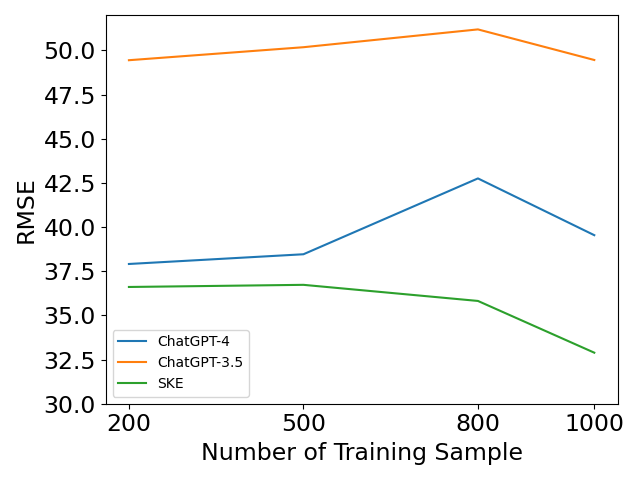
\includegraphics[width=0.3\linewidth]{figs/fraud-GPT-rmse.png}}
\hspace{0.001\linewidth}
\subfigure[Fraud: Macro F1]{\label{fig:fraud-gpt-f1}
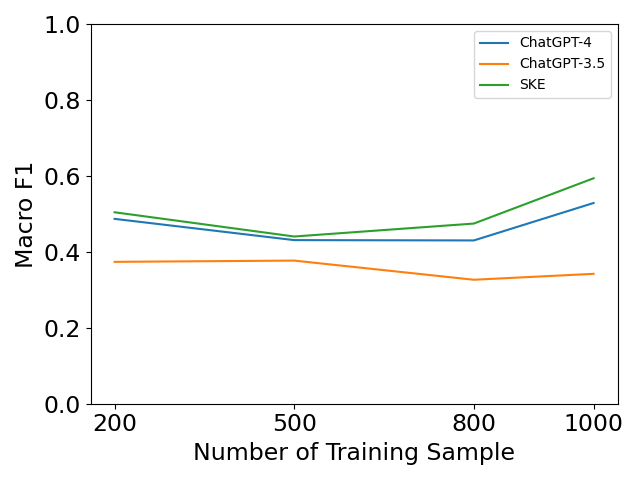
\includegraphics[width=0.3\linewidth]{figs/fraud-GPT-F1.png}}
\hspace{0.001\linewidth}
\subfigure[Fraud: Pearson]{\label{fig:fraud-gpt-p}
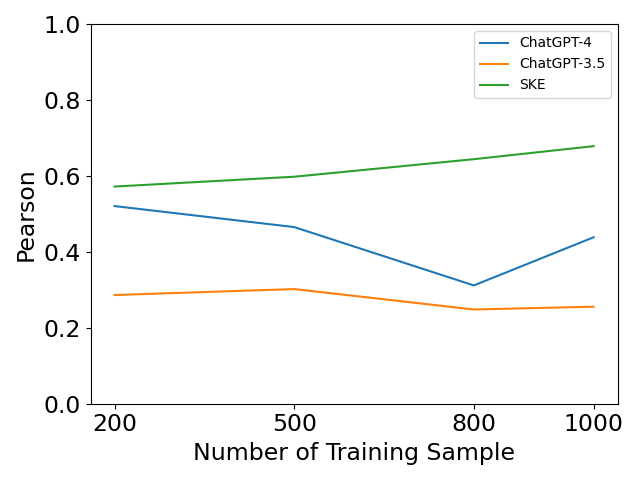
\includegraphics[width=0.3\linewidth]{figs/fraud-GPT-pearson.png}}
\vspace{-1em}


\vfill
\hspace{0.001\linewidth}
\subfigure[Intentional Injury: RMSE]{\label{fig:injure-gpt-rmse}
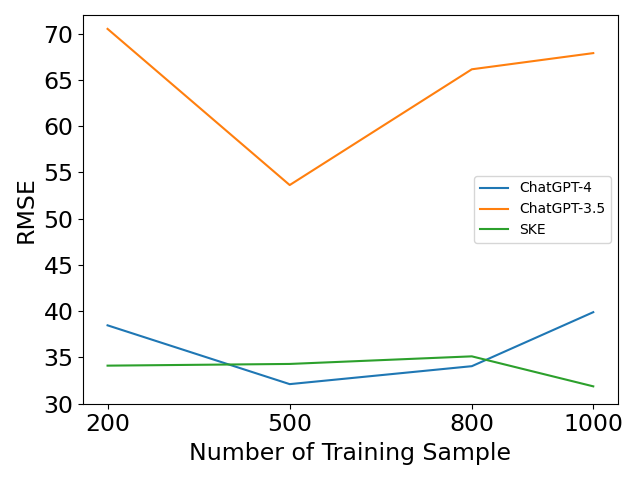
\includegraphics[width=0.3\linewidth]{figs/injure-GPT-rmse.png}}
\hspace{0.001\linewidth}
\subfigure[Intentional Injury: Macro F1]{\label{fig:injure-gpt-f1}
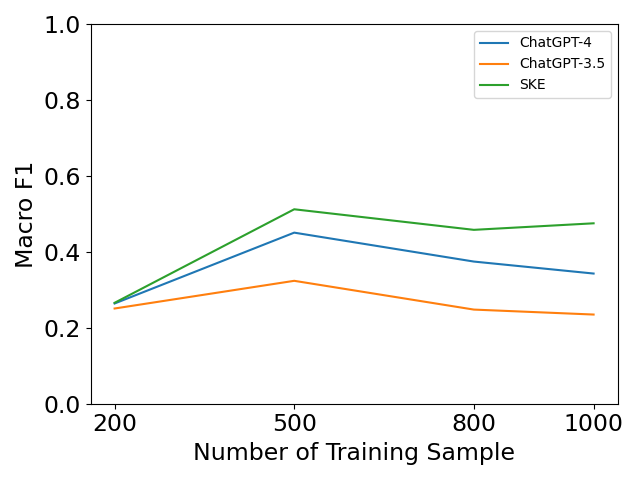
\includegraphics[width=0.3\linewidth]{figs/injure-GPT-f1.png}}
\hspace{0.001\linewidth}
\subfigure[Intentional Injury: Pearson]{\label{fig:injure-gpt-p}
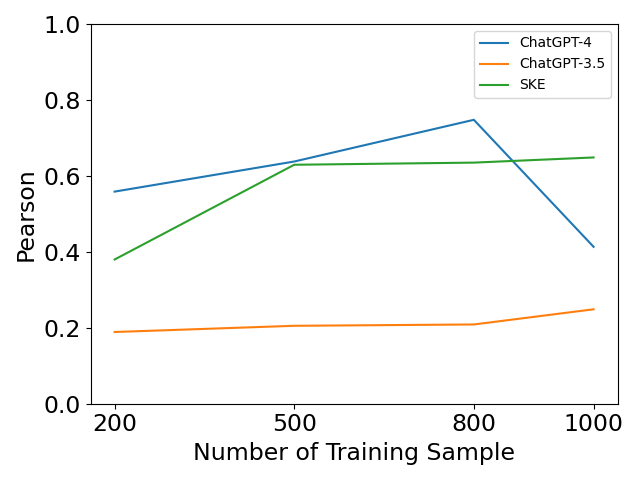
\includegraphics[width=0.3\linewidth]{figs/injure-GPT-pearson.png}}
    \vspace{-1em}
\caption{Comparison with LLMs. 
% \KZ{make fonts in the pics larger.}
}
\label{fig:gpt}
% \vspace{-1em}
\end{figure*}

\paragraph{Hyper-parameter Setting.}

For the proposed statute knowledge enhanced method, all learnable parameters are initialized by a standard normal distribution, and hidden vector dimensions $d$ with the same settings as previous work~\cite{neurjudge}. We utilize Adam optimizer with the learning rate $1\times 10^{-3}$. To reduce randomness, we take the average results from 5 times of experiments. 

We perform training and evaluation on a workstation with an Nvidia GeForce RTX 4090 GPU with 24 GB memory. 



% \begin{figure*}
% \vspace{-1em}

%     \centering
%     \subfigure[Fraud: MAE]{\label{fig:fraud-mae}
% 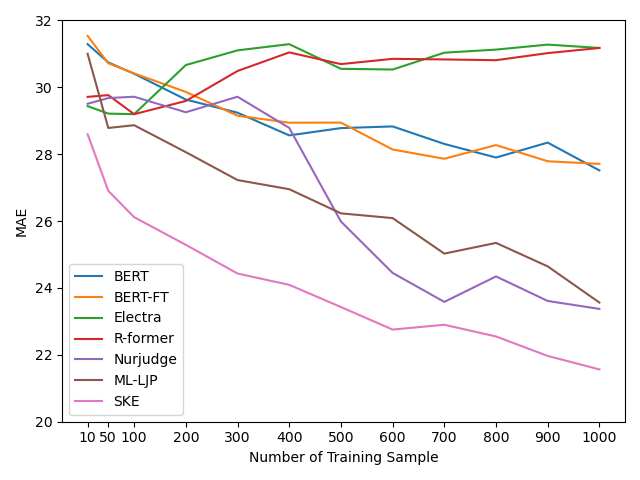
\includegraphics[width=0.22\linewidth]{latex/figs/fraud-mae.png}}
% % \vfill
% \hspace{0.001\linewidth}
% \subfigure[Fraud: RMSE]{\label{fig:fraud-rmse}
% \includegraphics[width=0.22\linewidth]{latex/figs/fraud-rmse.png}}
% \hspace{0.001\linewidth}
% \subfigure[Fraud: Macro F1]{\label{fig:fraud-f1}
% 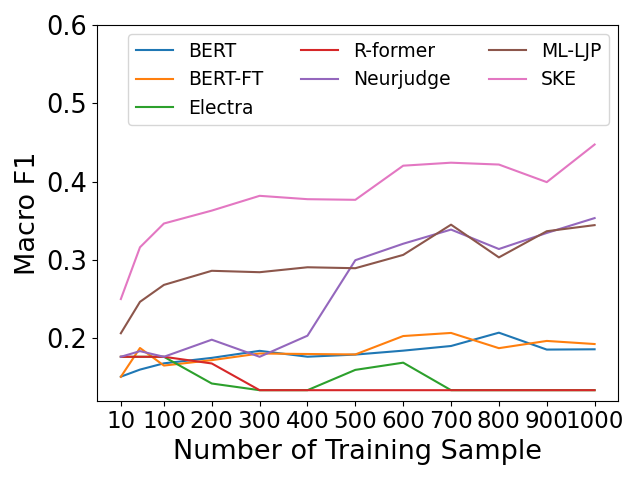
\includegraphics[width=0.22\linewidth]{latex/figs/fraud-F1.png}}
% \hspace{0.001\linewidth}
% \subfigure[Fraud: Pearson]{\label{fig:fraud-p}
% \includegraphics[width=0.22\linewidth]{latex/figs/fraud-pearson.png}}
% \vspace{-1em}

% \subfigure[II: MAE]{\label{fig:injure-mae}
% 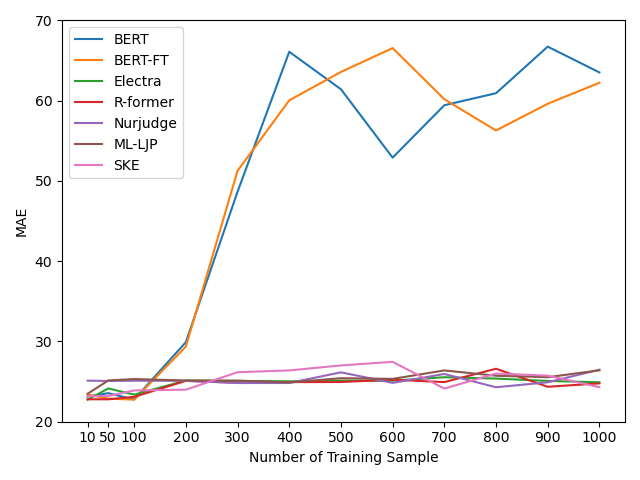
\includegraphics[width=0.22\linewidth]{latex/figs/injure-mae.png}}
% % \vfill
% \hspace{0.001\linewidth}
% \subfigure[II: RMSE]{\label{fig:injure-rmse}
% \includegraphics[width=0.22\linewidth]{latex/figs/injure-rmse.png}}
% \hspace{0.001\linewidth}
% \subfigure[II: Macro F1]{\label{fig:injure-f1}
% \includegraphics[width=0.22\linewidth]{latex/figs/injure-F1.png}}
% \hspace{0.001\linewidth}
% \subfigure[II: Pearson]{\label{fig:injure-p}
% \includegraphics[width=0.22\linewidth]{latex/figs/injure-pearson.png}}
%     \vspace{-1em}

% \subfigure[Robbery: MAE]{\label{fig:robbery-mae}
% 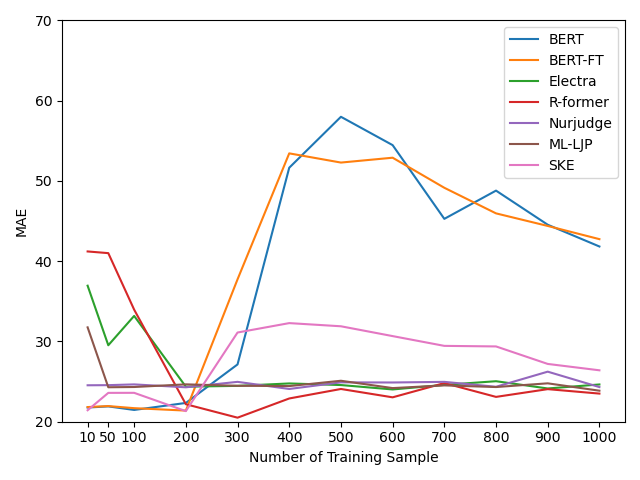
\includegraphics[width=0.22\linewidth]{latex/figs/robbery-mae.png}}
% % \vfill
% \hspace{0.001\linewidth}
% \subfigure[Robbery: RMSE]{\label{fig:robbery-rmse}
% \includegraphics[width=0.22\linewidth]{latex/figs/robbery-rmse.png}}
% \hspace{0.001\linewidth}
% \subfigure[Robbery: Macro F1]{\label{fig:robbery-f1}
% \includegraphics[width=0.22\linewidth]{latex/figs/robbery-F1.png}}
% \hspace{0.001\linewidth}
% \subfigure[Robbery: Pearson]{\label{fig:robbery-p}
% \includegraphics[width=0.22\linewidth]{latex/figs/robbery-pearson.png}}
%         \vspace{-1em}

% \subfigure[Arson: MAE]{\label{fig:arson-mae}
% 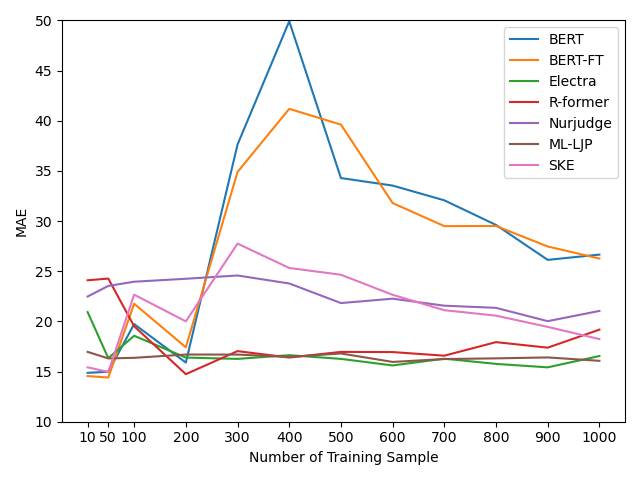
\includegraphics[width=0.22\linewidth]{latex/figs/arson-mae.png}}
% % \vfill
% \hspace{0.001\linewidth}
% \subfigure[Arson: RMSE]{\label{fig:arson-rmse}
% 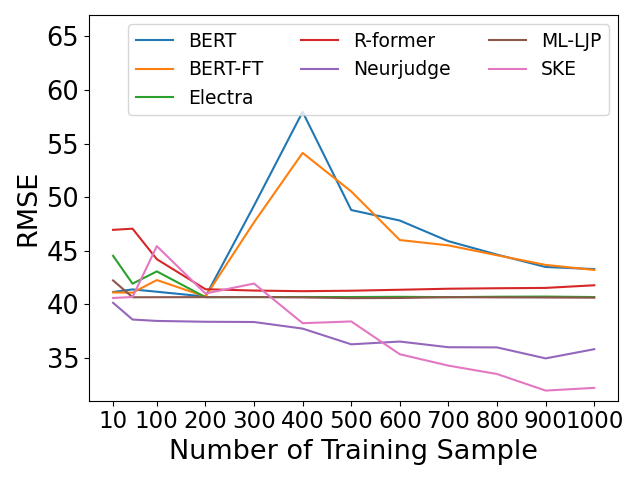
\includegraphics[width=0.22\linewidth]{latex/figs/arson-rmse.png}}
% \hspace{0.001\linewidth}
% \subfigure[Arson: Macro F1]{\label{fig:arson-f1}
% 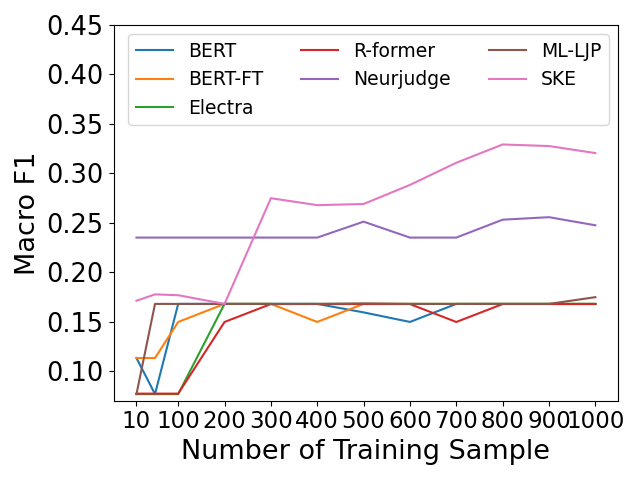
\includegraphics[width=0.22\linewidth]{latex/figs/arson-F1.png}}
% \hspace{0.001\linewidth}
% \subfigure[Arson: Pearson]{\label{fig:arson-p}
% 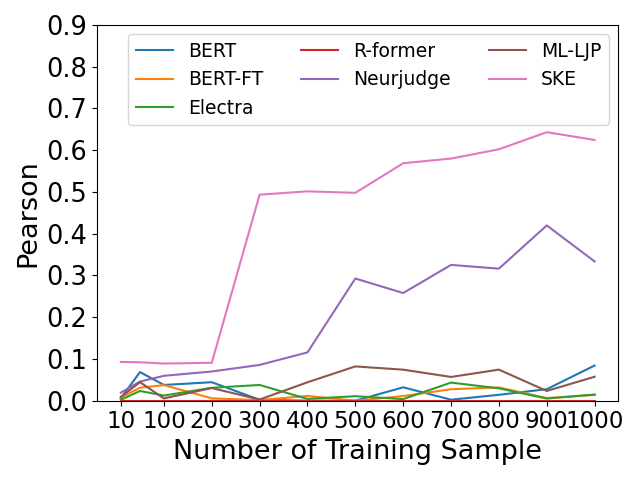
\includegraphics[width=0.22\linewidth]{latex/figs/arson-pearson.png}}
%     \vspace{-1em}

% \caption{Results on Four Different Laws. II denotes the intentional injury.
% \KZ{Fonts too small. Fonts in figs and tables must be at least 2/3 of the main text size.}}
% \label{fig:over}
% \vspace{-2em}
% \end{figure*}

\subsection{Comparisons among PTP Methods}

Table~\ref{fig:over} presents a comparison between previous representative methods and our proposed methods. 

Compared to the conventional methods, methods incorporating statute information significantly outperform their counterparts. This superiority is primarily attributed to conventional methods lacking the legal knowledge for accurate decision-making. This observation aligns with findings reported in previous studies.

Compared to methods that emphasize case relations, the proposed SKE method surpasses the R-former method in performance. Although R-former achieves a few good results in metrics such as MAE or RMSE, these advantages are minimal due to the narrow range of predicted penalty times across all cases. Pearson correlation results further corroborate this lack of relevance to the actual labels. This limitation may stem from these method dependencies on historical cases, which are restricted in the PTP problem.

Compared to methods leveraging statute information, the proposed SKE method outperforms the state-of-the-art ML-LJP method. This enhanced performance is credited to our application of the Law-Graph through transforming plain text legal information into a structured format, thereby facilitating easier comprehension by the models.

We evaluate the impact of training sample size. Initially, with fewer than 200 training cases, the proposed SKE method also demonstrates a weak correlation with human judgments. Then, the correlation strengthens as the training sample size increases to between 200 and 400 cases. Beyond 400 cases, the method strongly correlates with human judgments, which significantly outperforms other methods. These results suggest that our proposed SKE model is effective in scenarios with infrequent crimes or limited case examples.



\subsection{Comparison with Large Language Models}
With the development of Large Language Models (LLMs) that demonstrate good performance across various tasks~\cite{NEURIPS2020_1457c0d6,Katz2023GPT4PT, sun2023short}, it becomes imperative to assess the need for specialized task models in the PTP problem. We compare our proposed SKE method against two benchmark LLMs, ChatGPT-3.5 and ChatGPT-4~\cite{NEURIPS2022_b1efde53,DBLP:journals/corr/abs-2303-08774}, by conducting evaluations using fraud and intentional injury cases. Due to the usage limitation of ChatGPT, we selected a subset of 200 cases for each type of crime to serve as test instances, ensuring that these LLMs were provided with the same training samples for in-context learning utilized for the SKE method. The outcomes of these evaluations are detailed in Figure~\ref{fig:gpt}.

Our SKE method generally surpasses the performance of the ChatGPT models, showing particularly significant advantages over ChatGPT-3.5. Although ChatGPT-4 is a little bit better in a few points, its deployment is constrained by the requirement for billions of parameters and extensive training periods. In contrast, the SKE method requires only approximately 2000MB of memory and less than a day's training for each type of crime, presenting a more cost-effective solution. More importantly, the legal domain, especially courts, demands stringent data privacy measures that may not be readily achievable with ChatGPT. Our method offers a local processing advantage, ensuring enhanced protection of personal privacy, which is crucial for legal applications.

% \begin{figure}
%     \centering
%     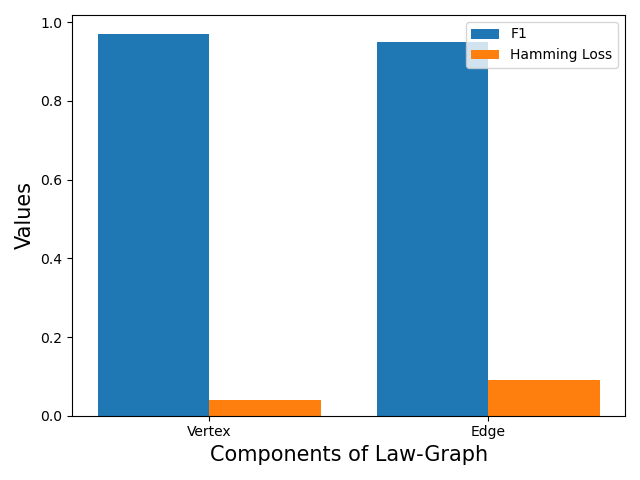
\includegraphics[width=0.8\linewidth]{latex/figs/eva.png}
%     \caption{Evaluation of constructed Law-Graphs.}
%     \label{fig:eva}
%     \Kaiqi{I think we don't need to use a figure. This figure can't make any comparison. Consider providing the numbers in the text.}
% \vspace{-1em}
% \end{figure}

\subsection{Quality Analysis of \lawgraph{s}}
The Law Graph quality directly influences the performance of the SKE method, underscoring the importance of evaluating its quality. To undertake this assessment, we randomly select 50 crimes from Chinese Criminal Law as a basis for comparison between the \lawgraph{} generated by our method (detailed in Section~\ref{con}) and those constructed by human experts. We simplify this comparison by framing it as a multi-label classification problem~\cite{6471714}, focusing on both the vertices and edges that comprise the Law Graph. The evaluation employs F1 scores and Hamming Loss as metrics to quantify the performance and accuracy of the constructed Law Graphs.

After experiments, we obtain 97.48\% F1 scores and 0.04 Hamming Loss for node comparison with labels; and 95.08\% F1 scores and 0.09 Hamming Loss for edge comparisons. The high F1 scores and low Hamming Loss values. Additionally, we conducted an error analysis to identify the sources of inaccuracies. These errors have two reasons: the misinterpretation of parallel words and the failure to accurately differentiate between leading elements and subsequent steps in statutory provisions.


